% Manuscript insertion fragment, not a standalone document.
% Requires amsmath, amssymb, and graphicx in the parent manuscript.
% Adjust the graphics path when copying into another project.
% Use figure* for a two-column paper; use figure for a single-column paper.
% The earlier Gaussian fragment is preserved in fig2_gaussian_manuscript.tex.
% The initial four-setting bounded version is in fig2_bounded_initial_manuscript.tex.

\paragraph{Sensitivity to partition resolution under bounded dependence.}
To study partition selection for a density satisfying the distributional
regularity assumptions of the theory, we consider
\begin{equation}
f_d(\mathbf{x})=1+0.7\cos\!\bigl(2\pi(x_1-x_2)\bigr),
\qquad \mathbf{x}\in[0,1]^d.
\label{eq:bounded-dependent-density}
\end{equation}
This density has uniform coordinate marginals but dependence between the
first two coordinates; the remaining coordinates are independent uniforms.
It satisfies $0.3\le f_d\le1.7$ and is Lipschitz on the cube with constant
$1.4\pi\sqrt{2}$, independently of $d$.
Its entropy is available analytically as
$H(f_d)=s-1-\log((1+s)/2)\approx-0.131623$ nats,
where $s=\sqrt{1-0.7^2}$.

We compare $d\in\{2,3,4,5\}$ at $n=10^5$ and
$n\in\{10^3,10^4,10^5,10^6\}$ at $d=2$.
We reuse five existing settings and add simulations at $d=3,4$ with new seeds.
There are seven distinct settings, with 100 independent repetitions for
$n\le10^5$ and 30 for $n=10^6$.
Figure~\ref{fig:bounded-ell} displays the common grid
$\mathcal{L}=\{1,\ldots,7\}$, also used for the new simulations.
For the reused settings, its RMSE minima agree with those over the full
archived candidate grids.
All resolutions within a repetition use the same dataset.
We compare the RMSE-minimizing resolution with the \emph{theory-selected}
resolution
\begin{equation}
\begin{aligned}
\ell_{\mathrm{th}}
&=\underset{\ell\in\mathcal{L}}{\operatorname{arg\,min}}
\left\{\ell^{-2}+\sqrt{\Lambda_{n,d,\delta}}
\left(\frac{\ell^d}{n}\right)^{1/4}\right\},\\
\Lambda_{n,d,\delta}
&=2d\log(2n+1)+\log(96/\delta),\qquad\delta=0.05.
\end{aligned}
\label{eq:bounded-theory-ell}
\end{equation}
This rule minimizes the dependence on $\ell$ in the displayed error bound;
the common positive factor $Kd$ does not affect the minimizer.
No coefficient is fitted to the observed errors, and no coverage filter is
used when identifying the empirical minima.

At $d=2$, the RMSE-minimizing resolution increases from $1$ to $2$ to $3$
to $4$ as $n$ increases from $10^3$ to $10^6$, while the minimum RMSE decreases.
The corresponding theory-selected resolutions are $2,2,3,3$.
At $n=10^5$, the empirical minima for $d=2,3,4,5$ occur at
$\ell=3,3,2,2$, respectively, compared with theoretical choices $3,2,2,1$.
Thus the choices agree in three of the seven distinct settings.
For the added $d=3$ setting, the theory-selected $\ell=2$ has RMSE
$0.04332$, close to the grid minimum $0.04019$ at $\ell=3$;
the added $d=4$ setting agrees at $\ell=2$.
These results illustrate sensitivity to partition resolution and the
distinction between minimizing an error bound and minimizing actual RMSE.
Although the density meets the distributional assumptions, this experiment
does not certify the theorem's finite-sample conditions involving the
unspecified constant $K_0$.

\begin{figure*}[t]
\centering
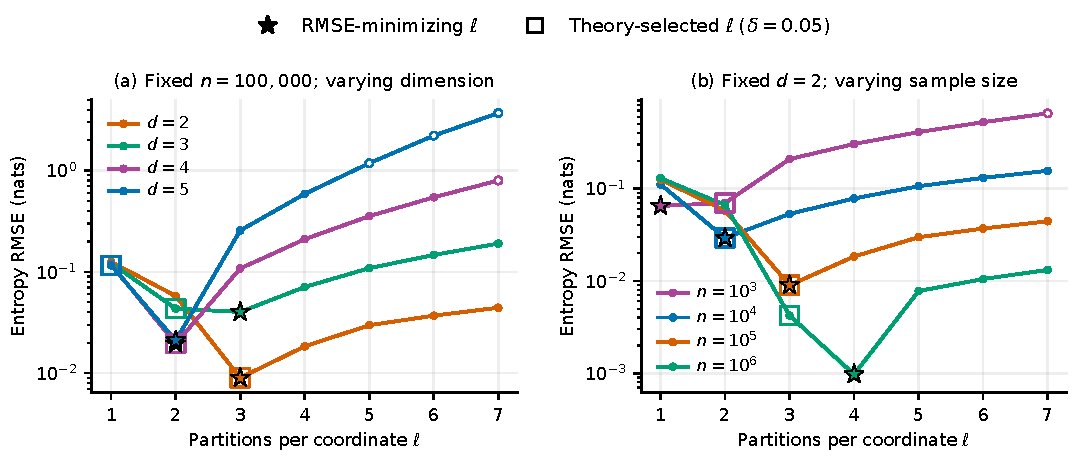
\includegraphics[width=\textwidth]{output/pdf/synthetic_bounded_fig2_extended_20261006/bounded_ell_rmse.pdf}
\caption{Entropy-estimation RMSE versus the number of partitions per coordinate
for the bounded dependent density in Eq.~\eqref{eq:bounded-dependent-density}.
(a) Fixed $n=10^5$ and varying $d$.
(b) Fixed $d=2$ and varying $n$.
Results use 100 repetitions for $n\le10^5$ and 30 for $n=10^6$;
shading denotes pointwise 95\% bootstrap intervals from 2,000 resamples.
Stars mark the RMSE-minimizing $\ell$ over the displayed grid, using the same
repetitions as the curves. Squares mark the theory-selected $\ell$ from
Eq.~\eqref{eq:bounded-theory-ell}.
Hollow circles indicate incomplete coverage in at least one repetition;
all starred candidates have full coverage in every repetition.
The shared setting $(n,d)=(10^5,2)$ appears in both panels.}
\label{fig:bounded-ell}
\end{figure*}
